% !TEX encoding = UTF-8
% !TEX program = xelatex
\documentclass[12pt,a4paper]{article}
\usepackage[paperwidth=210mm, paperheight=297mm, left=0.75in, right=0.75in, bottom=1in, top=1in]{geometry}
\usepackage{polyglossia}
\setdefaultlanguage[babelshorthands]{italian}
\usepackage{fontspec}
\usepackage{graphicx}
\usepackage{blindtext}
\usepackage{wrapfig}

\frenchspacing
\makeindex

\begin{document}
\title{\vspace{-70pt}COBE}
\author{Enrico Angeli}
\date{}
\maketitle
\pagestyle{empty}
\thispagestyle{empty}


\section*{Storia}
\label{storia}
\begin{wrapfigure}{r}{0.35\textwidth}
  \vspace{-10pt}
  \begin{center}
    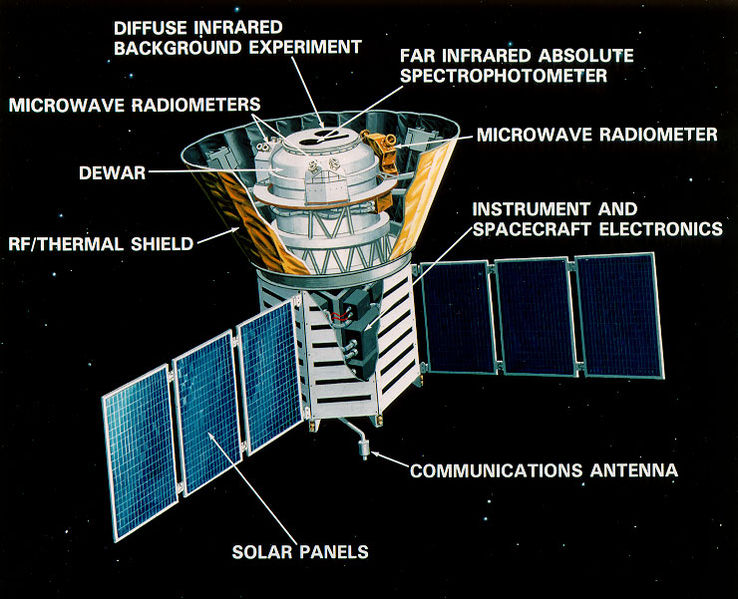
\includegraphics[width=0.30\textwidth]{satellite}
  \end{center}
  \vspace{-20pt}
\end{wrapfigure}
Il satellite \textbf{COBE} (COsmic Background Explorer) fu lanciato dalla NASA il \textbf{18 novembre 1989}, dopo 15 anni dalla sua proposta. La sua missione era di misurare lo spettro della Radiazione cosmica di fondo a microonde e di cercare eventuali disuniformità in questa radiazione.

Le sue misure sono alla base della cosmologia moderna poiché hanno permesso di misurare con precisione la radiazione cosmica di fondo.

\section*{Osservazioni}
\label{osservazioni}

Il satellite COBE fu lanciato dalla Vandenberg Air Force Base a Lompoc, California, il 18 novembre 1989, tramite il veicolo di lancio Delta 5000.
La sua missione prevedeva un viaggio di circa 4 anni, orbitando attorno alla terra a una distanza di 900.2 km a un periodo orbitale di 103 minuti. 

Il satellite disponeva a bordo di tre strumentazioni principali:

\begin{itemize}
\item DIRBE: Diffuse InfraRed Background Experiment, un rivelatore a infrarossi a più lunghezze d'onda usato per mappare l'emissione di polveri;

\item FIRAS: Far-InfraRed Absolute Spectrophotometer, uno spettrofotometro usato per misurare lo spettro della Radiazione Cosmica di Fondo (CMB)

\item DMR: Differential Microwave Radiometer: uno strumento a microonde usato per mappare le variazione (o le anisotropie) nella Radiazioni Cosmica di Fondo (CMB)

\end{itemize}

\textbf{John Mather} e \textbf{George Smoot} hanno successivamente studiato le misurazioni ottenute dalle rilevazioni apportate dal satellite COBE, dimostrando che la Radiazione Cosmica di Fondo ha uno spettro quasi perfettamente di \textbf{corpo nero}, che emette a una temperatura di (2,725±0,0002)K, corrispondente all'eccesso di temperatura che Penzias e Wilson non riuscivano a spiegare. Tale temperatura risulta sempre la stessa, indipendentemente dalla direzione in cui la si osserva, ma presenta comunque piccole deviazioni, dette \textbf{anisotropie}, in una parte su centomila. 

Queste due proprietà hanno confermato la teoria del Big Bang.

\section*{Curiosità}
\label{curiosit}

John Mather e George Smoot sono stati insigniti del premio Nobel per la fisica nel 2006, grazie alle loro scoperte sulle anisotropie.

La scoperta delle anisotropie fu commentata da Stephen Hawking come ``\emph{la più grande scoperta scientifica del secolo}''.


\end{document}